%!Mode::"UTF-8"
\documentclass[12pt]{article}

% 页面设置
\usepackage{geometry}
\geometry{left=2.5cm, right=2.5cm, top=2.5cm, bottom=2.5cm}
\usepackage{graphicx}
\usepackage{ctex}
\usepackage{fontspec}
\usepackage{setspace}

% 代码设置
\usepackage{listings}
\usepackage{color}
\setmonofont{Consolas}
\definecolor{listing}{gray}{0.97}
\lstset{
	backgroundcolor=\color{listing},
	basicstyle=\footnotesize,
	numbers=left,
	numberstyle=\footnotesize,
	stepnumber=1,
	aboveskip={0.5\baselineskip},
	belowskip={0.5\baselineskip},
	columns=fullflexible,
	breaklines=true,
	breakatwhitespace=true,
	frame=single,
	basicstyle=\ttfamily,
	numberstyle=\ttfamily,
	tabsize=2
}

% 字体设置
\setmainfont{Times New Roman}
\setCJKmainfont{SimSun}
\setCJKsansfont{SimHei}

% 表格设置
\usepackage{makecell}
\newcommand{\addcell}[2][4]{\makecell{\zihao{#1}\textsf{#2}}}
\usepackage{titlesec}
\usepackage{booktabs}
\usepackage{tabularx}

% 设置图注、表注
\usepackage{caption}
\usepackage{bicaption}
\captionsetup{labelsep=quad, font={small, bf}, skip=2pt}
\DeclareCaptionOption{english}[]{
    \renewcommand\figurename{Fig.}
    \renewcommand\tablename{Table}
}
\captionsetup[bi-second]{english}

% 设置页眉
\usepackage{fancyhdr}
\pagestyle{fancy}
\fancypagestyle{preContent}{
    \fancyhead[L]{\zihao{-5} 物理化学实验}
    \fancyhead[C]{\zihao{-5} 实验六\ \ 溶液表面吸附的测定}
    \fancyhead[R]{\zihao{-5} 1800011828\ 王宇哲}
}
\pagestyle{preContent}

%	设置首页页眉页脚
\fancypagestyle{plain}{
	\fancyhead[L]{\zihao{-5} 物理化学实验}
	\fancyhead[C]{\zihao{-5} 实验六\ \ 溶液表面吸附的测定}
	\fancyhead[R]{\zihao{-5} 1800011828\ 王宇哲}
	\cfoot{}
}

% 设置标题格式
\titleformat*{\section}{\zihao{4}\sffamily}
\titleformat*{\subsection}{\zihao{-4}\sffamily}
\titleformat*{\subsubsection}{\zihao{-4}\sffamily}
\titlespacing*{\section}{0pt}{10pt}{10pt}
\titlespacing*{\subsection}{0pt}{10pt}{5pt}
\titlespacing*{\subsubsection}{0pt}{10pt}{5pt}

% 设置引用格式
\usepackage[super,round,comma,compress]{natbib}

\usepackage{amsmath}
\usepackage{amssymb}

%设置封面
\begin{document}
    % 标题页
    \begin{titlepage}
    	% 页眉
    	\thispagestyle{plain}
        % 图片
        \begin{figure}[h]
            \centering
            \includegraphics{pku.png}
        \end{figure}
        \vspace{24pt}
        % 标题
        \centerline{\zihao{-0} \textsf{物理化学实验报告}}
        \vspace{40pt} % 空行
        \begin{center}
            \begin{tabular}{cp{9.5 cm}}
                % 题目
                \addcell[2]{题目:\ } & \addcell[2]{溶液表面吸附的测定} \\
                \cline{2-2}
            \end{tabular}
        \end{center}
        \vspace{20pt} % 空行
        \begin{center}
            \doublespacing
            \begin{tabular}{cp{5cm}}
                % 姓名
                \addcell{姓\phantom{空格}名:\ } & \addcell{王宇哲} \\
                \cline{2-2}
                % 学号
                \addcell{学\phantom{空格}号:\ } & \addcell{1800011828}\\
                \cline{2-2}
                % 组别
                \addcell{组\phantom{空格}别:\ } & \addcell{11组3号} \\
                \cline{2-2}
                % 实验日期
                \addcell{实验日期:\ } & \addcell{2020.11.4}\\
                \cline{2-2}
                % 室温
                \addcell{室\phantom{空格}温:\ } & \addcell{293.05\ K}\\
                \cline{2-2}
                % 大气压强
                \addcell{大气压强:\ } & \addcell{102.21\ kPa}\\
                \cline{2-2}
            \end{tabular}
            \begin{tabular*}{\textwidth}{c}
                \\ % 这是空行
                \\ % 这是空行
                \\ % 这是空行
                \\ % 这是空行
                \hline % 分割线
            \end{tabular*}
        \end{center}
        % 摘要
        \textsf{摘\ \ 要}\ \ 本实验使用最大气泡压力法和吊片法测定纯水和8个不同浓度正丁醇溶液的表面张力,作出了正丁醇水溶液的$\gamma-{\rm lg}c$等温曲线,通过最大气泡压力法计算了正丁醇分子的饱和吸附量$\Gamma_{\infty}=(5.6\pm 0.5)\times10^{-6}\ \ {\rm mol\cdot m^{-2}}$,分子吸附面积$q=(0.30\pm 0.03)\ \ {\rm nm^{2}}$,$c=0.329\ \ {\rm mol\cdot L^{-1}}$的正丁醇溶液分子实际面积$q_{c}=(0.27\pm 0.03)\ \ {\rm nm^{2}}$。通过吊片法计算$\Gamma_{\infty}=(5.0\pm 0.5)\times10^{-6}\ \ {\rm mol\cdot m^{-2}}$,$q=(0.33\pm 0.03)\ \ {\rm nm^{2}}$,$c=0.329\ \ {\rm mol\cdot L^{-1}}$的正丁醇溶液$q_{c}=(0.30\pm 0.03)\ \ {\rm nm^{2}}$。探讨了造成实验误差的原因。
        \\
        \\
        % 关键字
        \textsf{关键词}\ \ 最大气泡压力法;吊片法;表面张力;Gibbs吸附公式;饱和吸附
    \end{titlepage}

    \section{引言}
	略
               
\vbox{}        
    \section{实验部分}
    	\subsection{仪器和药品}
    	\subsubsection{仪器}
    	最大气泡压力法表面张力测定装置,QBZY-2型表面张力仪,恒温水浴装置。
    	\subsubsection{试剂}
    	纯水,$8$种不同浓度的正丁醇溶液(浓度分别为$0.0218\ \ {\rm M}$、$0.0547\ \ {\rm M}$、$0.111\ \ {\rm M}$、$0.220\ \ {\rm M}$、$0.329\ \ {\rm M}$、$0.439\ \ {\rm M}$、$0.550\ \ {\rm M}$、$0.740\ \ {\rm M}$)。
\vbox{}
    	 \subsection{实验内容\citealp{physchemlab}}
			\subsubsection{最大气泡压力法测量纯水表面张力}
	调节恒温槽,将温度设定为$30.00\ \ {\rm ^{\circ}C}$。检查并使用洗耳球清洗毛细管,将$\sim2 \ \ {\rm mL}$纯水装入试管,调整好毛细管的位置,使毛细管尖端与溶液液面相切。\par 
	打开安全阀,关闭调节活塞,记录无压力时压力计左右两管液柱高度$h_{L}$、$h_{R}$及液柱高度差$\Delta h_{0}=h_{R}-h_{L}$,重复读取3次,取平均值作为压力计的零点位置。\par 
	关闭活塞和安全阀,通过双联球给缓冲瓶加压。小心调节活塞的针阀,使气泡从产生到爆裂的时间大于$8\ \ {\rm s}$。当气泡逸出毛细管尖端时,压力计的水柱差会突然下降,记录下降前的水柱最大高度差$\Delta h$,重复3次,计算$\Delta h$的平均值。
			\subsubsection{最大气泡压力法测量正丁醇表面张力}
	检查并清洗毛细管,依次测量8个不同浓度的正丁醇溶液的压力差值,每次测量前用新的溶液将毛细管内壁和试管洗涤$2\sim 3$次。关闭活塞,将不同浓度的正丁醇溶液$\sim2 \ \ {\rm mL}$装入试管,调整毛细管的位置,打开安全阀,读取压力计零点位置;关闭安全阀,调节活塞针阀,测定$\Delta h$。每种溶液进行2次测量,计算$\Delta h$的平均值。
		
			\subsubsection{吊片法测量表面张力}
	用镊子夹取白金板,用去离子水清洗,随后用酒精灯灼烧白金板,保持白金板与水平面呈$45^{\circ}$角进行,直至白金板变红,将白金板挂在挂钩上冷却。\par 
	将待测溶液加入样品皿中,置于升降样品台上;将处理好并已经冷却的白金板挂在吊钩上,观察显示屏示数是否为0,若不为0则按“去皮”键作清零处理;关上有机玻璃门,按“手动/自动”键将仪器调至自动状态;按“向上”键开始表面张力的自动测定,待显示屏数值稳定后,读取相应的表面张力$\gamma$和仪器显示的温度$t$;测量完成后,按“向下”键将样品与白金板脱离。每个样品重复3次,计算$\gamma$的平均值。

\vbox{}
 \section{数据与结果}
 \subsection{实验数据记录及处理}
 \subsubsection{最大气泡压力法测量纯水表面张力}
读取无压力时压力计左右两管液柱高度$h_{L}$、$h_{R}$及液柱高度差$\Delta h_{0}=h_{R}-h_{L}$,即压力计无压力时的零点位置,结果示于\textbf{表1}。
\begin{table}[h]
	\centering
	\zihao{5}
	\bicaption{压力计零点位置测量数据}{Pressure gauge zero position measurement data}
	\begin{tabular}{cccc}
		\toprule
		编号 & $h_{L}/{\rm cm}$ & $h_{R}/{\rm cm}$ & $\Delta h_{0}/{\rm cm}$ \\
		\midrule
		1 & 16.58 & 16.54 & -0.04 \\
		2 & 16.59 & 16.57 & -0.02\\
		3 & 16.58 & 16.55 & -0.03\\
		\bottomrule
	\end{tabular}
\end{table}
\par
根据\textbf{表1}数据,计算$\Delta h_{0}$的平均值为
$$\Delta h_{0}=-0.03\ \ {\rm cm}
$$
考虑到$\Delta h_{0}$的标准偏差
$$
\sigma_{\Delta h_{0}}=\sqrt{\frac{0.01^{2}+0.01^2}{3-1}} \ \ {\rm cm}=0.01\ \ {\rm cm}
$$
远小于压力计的最小分度$0.1\ \ {\rm cm}$,因此可以认为压力计零点位置在读数过程中未发生改变,数据的微小差异来源于估读时的偶然误差。根据以上事实,后续测量时读取零点位置只读取一次,从而一定程度上简化了实验过程,并且可以认为该操作引入的实验误差几乎可以忽略不计。\par
调节活塞的针阀,通过最大气泡压力法测量纯水的表面张力,记录压力计左右两管液柱高度$h_{L}$、$h_{R}$及液柱高度差$\Delta h^{\prime}=h_{R}-h_{L}$,各项测量数据示于\textbf{表2}。
\begin{table}[h]
	\centering
	\zihao{5}
	\bicaption{最大气泡压力法测量纯水表面张力数据}{Measurement data of surface tension of water via maximum bubble pressure method}
	\begin{tabular}{cccc}
		\toprule
		编号 & $h_{L}/{\rm cm}$ & $h_{R}/{\rm cm}$ & $\Delta h^{\prime}/{\rm cm}$ \\
		\midrule
		1 & 11.50 & 21.54 & 10.04 \\
		2 & 11.50 & 21.58 & 10.08\\
		3 & 11.52 & 21.57 & 10.05\\
		\bottomrule
	\end{tabular}
\end{table}
\par 
计算$\Delta h^{\prime}$的平均值为
$$
\Delta h^{\prime}=\frac{10.04+10.08+10.05}{3}\ \ {\rm cm} =10.06\ \ {\rm cm}
$$
平均值的标准偏差
$$
\sigma_{\Delta h^{\prime}}=\sqrt{\frac{(10.04-10.09)^{2}+(10.08-10.09)^{2}+(10.05-10.09)^{2}}{3-1}}=0.04\ \ {\rm cm}
$$
\par 
考虑到压力计零点修正,计算实际的液柱高度差
$$\Delta h=\Delta h^{\prime}-\Delta h_{0} =10.09\ \ {\rm cm}$$
标准偏差$\sigma_{\Delta h}=\sigma_{\Delta h^{\prime}}$,故实际的液柱高度差
$$
\Delta h=(10.09\pm 0.04)\ \ {\rm cm}
$$


 \subsubsection{最大气泡压力法测量正丁醇表面张力}
 用最大气泡压力法依次测量8个不同浓度的正丁醇溶液的表面张力。检查并清洗毛细管,用待测正丁醇溶液润洗试管。将$\sim 2\ \ {\rm mL}$不同浓度的正丁醇溶液装入试管,调整好毛细管的位置,使毛细管尖端与溶液液面刚好相接触。打开安全阀,关闭调节活塞,读取压力计零点位置,记录压力计左右两管液柱高度$h_{L}$、$h_{R}$及液柱高度差$\Delta h_{0}$。关闭活塞和安全阀,小心调节活塞针阀,通过最大气泡压力法测量不同浓度的正丁醇溶液的表面张力,记录压力计左右两管液柱高度$h_{L}$、$h_{R}$及液柱高度差$\Delta h^{\prime}$。每个样品测2次,计算$\Delta h^{\prime}$的平均值。考虑压力计零点修正,计算实际的液柱高度差
 $$
 \Delta h=\Delta h^{\prime}-\Delta h_{0}
 $$
 其中$\delta h^{\prime}$取每种浓度正丁醇溶液2次测定的平均值。$\Delta h$的有效数字位数根据由计算得到的标准偏差确定,以$c_{\rm BuOH}=0.0218\ \ {\rm mol\cdot L^{-1}}$为例,有
 $$
 \sigma_{\Delta h}=\sqrt{\frac{(9.59-9.58)^{2}}{2-1}}\ \ {\rm cm}=0.01\ \ {\rm cm}
 $$
 其他各正丁醇浓度下的标准偏差可以类似地计算。以上各项数据示于\textbf{表3},其中$c_{\rm BuOH}$为正丁醇溶液的浓度。
 \begin{table}[h]
 	\centering
 	\zihao{5}
 	\bicaption{最大气泡压力法测量正丁醇表面张力数据}{Measurement data of surface tension of n-BuOH via maximum bubble pressure method}
 	\begin{tabular}{cccccc}
 		\toprule
 		$c_{\rm BuOH}/{\rm mol\cdot L^{-1}}$ & 编号 & $h_{L}/{\rm cm}$ & $h_{R}/{\rm cm}$ & $\Delta h_{0}$ or $\Delta h^{\prime}/{\rm cm}$ & $\Delta h/{\rm cm}$  \\
 		\midrule
~      & 零点&16.59 & 16.52 & -0.07 & ~ \\
0.0218 & 1  &11.73 & 21.32 & 9.59 & 9.65$\pm$0.01 \\
~      & 2  &11.75 & 21.33 & 9.58 & \\
 		\midrule
~      & 零点&16.59 & 16.55 & -0.04 & ~ \\
0.0547 & 1  &12.19 & 20.85 & 8.66 & 8.70$\pm$0.01\\
~      & 2  &11.75 & 21.33 & 8.65 & \\
\midrule
~      & 零点&16.59 & 16.54& -0.05 & ~ \\
0.111 & 1  &12.69 & 20.33 & 7.64 & 7.67$\pm$0.02\\
~      & 2  &12.72 & 20.33 & 7.61 & ~ \\
\midrule
~      & 零点&16.58 & 16.55 & -0.03 & ~ \\
0.220 & 1  &13.28 & 19.79 & 6.51 & 6.55$\pm$0.01\\
~      & 2  &13.28 & 19.81 & 6.53 & ~ \\
\midrule
~      & 零点&16.59 & 16.56 & -0.03 & ~ \\
0.329 & 1  &13.69 & 19.40 & 5.71 & 5.75$\pm$0.01\\
~      & 2  &13.69 & 19.41 & 5.72 & \\
\midrule
~      & 零点&16.59 & 16.56 & -0.03 & ~ \\
0.439 & 1  &13.97 & 19.13 & 5.16 & 5.19$\pm$0.01\\
~      & 2  &13.96 & 19.12 & 5.16 & \\
\midrule
~      & 零点&16.57 & 16.55 & -0.02 & ~ \\
0.550 & 1  &14.22 & 18.89 & 4.67 & 4.68$\pm$0.01\\
~      & 2  &14.21 & 18.89 & 4.66 & \\
\midrule
~      & 零点&16.59 & 16.56 & -0.03 & ~ \\
0.740 & 1  &14.49 & 18.63 & 4.14 & 4.17$\pm$0.01\\
~      & 2  &14.49 & 18.62 & 4.13 & \\
 		\bottomrule
 	\end{tabular}
 \end{table}
\par 
 
 \subsubsection{吊片法测量表面张力}
 用吊片法依次测量纯水和8个不同浓度的正丁醇溶液的表面张力。每个样品测3次,每次测量时保持QBZY-2型表面张力仪显示的温度$t$在$27.6\ \ {\rm ^{\circ}C}$附近,读取仪器显示的表面张力$\gamma$,计算表面张力$\gamma$的平均值$\overline{\gamma}$。。$\overline{\gamma}$的有效数字位数根据由计算得到的标准偏差确定,以纯水为例,有
 $$
 \sigma_{\overline{\gamma}}=\sqrt{\frac{(70.66-70.63)^{2}+(70.65-70.63)^{2}+(70.58-70.63)^{2}}{3-1}}\ \ {\rm mN\cdot m^{-1}}=0.04\ \ {\rm mN\cdot m^{-1}}
 $$
 其他各正丁醇浓度下的标准偏差可以类似地计算。各项数据示于\textbf{表4}。
 \begin{table}[h]
	\centering
	\zihao{5}
	\bicaption{吊片法测量表面张力数据}{Measurement data of surface tension via hanging-piece method}
	\begin{tabular}{cccc}
		\toprule
		$c_{\rm BuOH}/{\rm mol\cdot L^{-1}}$ & 编号 & $\gamma /{\rm mN\cdot m^{-1}}$  & $\overline{\gamma}/{\rm mN\cdot m^{-1}}$  \\
		\midrule
~      & 1&70.66 & ~ \\
0(纯水) & 2  & 70.65 & 70.63$\pm$0.04\\
~      & 3  &70.58 &  \\
\midrule
~      & 1  &60.26 & ~ \\
0.0218 & 2  &60.54 & 60.1$\pm$0.5\\
~      & 3  &59.56 &  \\
\midrule
~      & 1  &58.63 & ~ \\
0.0547 & 2  &58.34 & 58.5$\pm$0.1\\
~      & 3  &58.50 &  \\
\midrule
~      & 1  &53.56 & ~ \\
0.111  & 2  &53.55 & 53.7$\pm$0.3\\
~      & 3  &54.11 &  \\
\midrule
~      & 1  &46.36 & ~ \\
0.220  & 2  &46.20 & 46.3$\pm$0.1\\
~      & 3  &46.47 &  \\
\midrule				
~      & 1  &43.14 & ~ \\
0.329  & 2  &43.47 & 43.4$\pm$0.2\\
~      & 3  &43.60 &  \\
\midrule		
~      & 1  &40.60 & ~ \\
0.439  & 2  &40.61 & 40.7$\pm$0.2\\
~      & 3  &40.99 &  \\
\midrule	
~      & 1  &35.60 & ~ \\
0.550  & 2  &37.10 & 36.2$\pm$0.8\\
~      & 3  &35.97 &  \\
\midrule	
~      & 1  &30.10 & ~ \\
0.740  & 2  &31.67 & 32$\pm$2\\
~      & 3  &34.53 &  \\
		\bottomrule
	\end{tabular}
\end{table}
\par 
 
 

 \subsection{数据处理结果与分析}
 \subsubsection{各浓度正丁醇水溶液的$\gamma$值}
 根据最大气泡压力法的实验原理,对于同一根毛细管,溶液表面张力$\gamma$与压力计左右两管液柱高度差$\Delta h$成正比。记纯水的表面张力为$\gamma_{\rm H_{2}O}$,纯水对应的压力计左右两管液柱高度差为$\Delta h_{\rm H_{2}O}$,则有
 $$
 \frac{\gamma_{\rm H_{2}O}}{\gamma}=\frac{\Delta h_{\rm H_{2}O}}{\Delta h}
 $$
 即
 $$
 \gamma=\frac{\gamma_{\rm H_{2}O} \Delta h}{\Delta h_{\rm H_{2}O}}
 $$
 \par 
 查阅手册\citealp{crc}得$30\ \ {\rm ^{\circ }C}$以下纯水的表面张力$\gamma_{\rm H_{2}O}=71.20\ \ {\rm mN\cdot m^{-1}=0.07120\ \ {\rm J\cdot m^{-2}}}$,实验测得对应的液柱高度差$\Delta h_{\rm H_{2}O}=10.09\ \ {\rm cm}$,对于各浓度正丁醇水溶液,将上述数据及实验测得的液柱高度差$\Delta h$代入公式中,即可计算得到各浓度正丁醇水溶液的表面张力$\gamma$。\par 
 以$c_{\rm BuOH}=0.0218\ \ {\rm mol\cdot L^{-1}}$为例,实验测得$\Delta h=9.65 \ \ {\rm cm}$,故计算
 $$
 \gamma=\frac{0.07120\ \ {\rm J\cdot m^{-2}} \times 9.65 \ \ {\rm cm}}{10.09\ \ {\rm cm}}=0.06810\ \ {\rm J\cdot m^{-2}}
 $$
 取$\sigma_{\Delta h}=0.01\ \ {\rm cm}$,$\sigma_{\Delta h_{\rm H_{2}O}}=0.01\ \ {\rm cm}$,则$\gamma$的标准偏差
 $$
 \sigma_{\gamma}=\frac{\gamma_{\rm H_{2}O}}{\Delta h_{\rm H_{2}O}}\sqrt{\sigma_{\Delta h}^{2}+(\frac{\Delta h}{\Delta h_{\rm H_{2}O}} \sigma_{\Delta h_{\rm H_{2}O}})^{2}}=0.00010\ \ {\rm J\cdot m^{-2}}
 $$
 故$$
 \gamma=(0.06810\pm 0.00010)\ \ {\rm J\cdot m^{-2}}
 $$
 为便于后续数据处理,多保留了一位。其他各浓度正丁醇水溶液的$\gamma$值可以类似地计算,计算结果示于\textbf{表5}。
 \begin{table}[h]
 	\centering
 	\zihao{5}
 	\bicaption{不同浓度正丁醇水溶液表面张力$\gamma$计算结果}{Calculation results of $\gamma$ of n-BuOH aqueous solution}
 	\begin{tabular}{ccc}
 		\toprule
 		$c_{\rm BuOH}/{\rm mol\cdot L^{-1}}$ & $\Delta h / {\rm cm}$ & $\gamma/{\rm J\cdot m^{-2}}$\\
 		\midrule
 		0.0218 & 9.65 & 0.06810$\pm$0.00010 \\
 		0.0547 & 8.70 & 0.06139$\pm$0.00009\\
 		0.111 & 7.67 &  0.05377$\pm$0.00009\\
 		0.220 & 6.55 & 0.04601$\pm$0.00008\\
 		0.329 & 5.75 & 0.04057$\pm$0.00008\\
 		0.439 & 5.19 & 0.03662$\pm$0.00008\\
 		0.550 & 4.68 & 0.03302$\pm$0.00008\\
 		0.740 & 4.17 & 0.02942$\pm$0.00008\\
 		\bottomrule
 	\end{tabular}
 \end{table}
\subsubsection{正丁醇水溶液$\gamma-{\rm lg}c$等温曲线与饱和吸附量$\Gamma_{\infty}$}
根据\textbf{表4}数据,使用python matplotlib绘制正丁醇水溶液$\gamma-{\rm lg}c$关系散点图,并光滑连接各散点,作出正丁醇水溶液$\gamma-{\rm lg}c$等温曲线,如\textbf{图1}所示。
\begin{figure}[h]
	\centering
	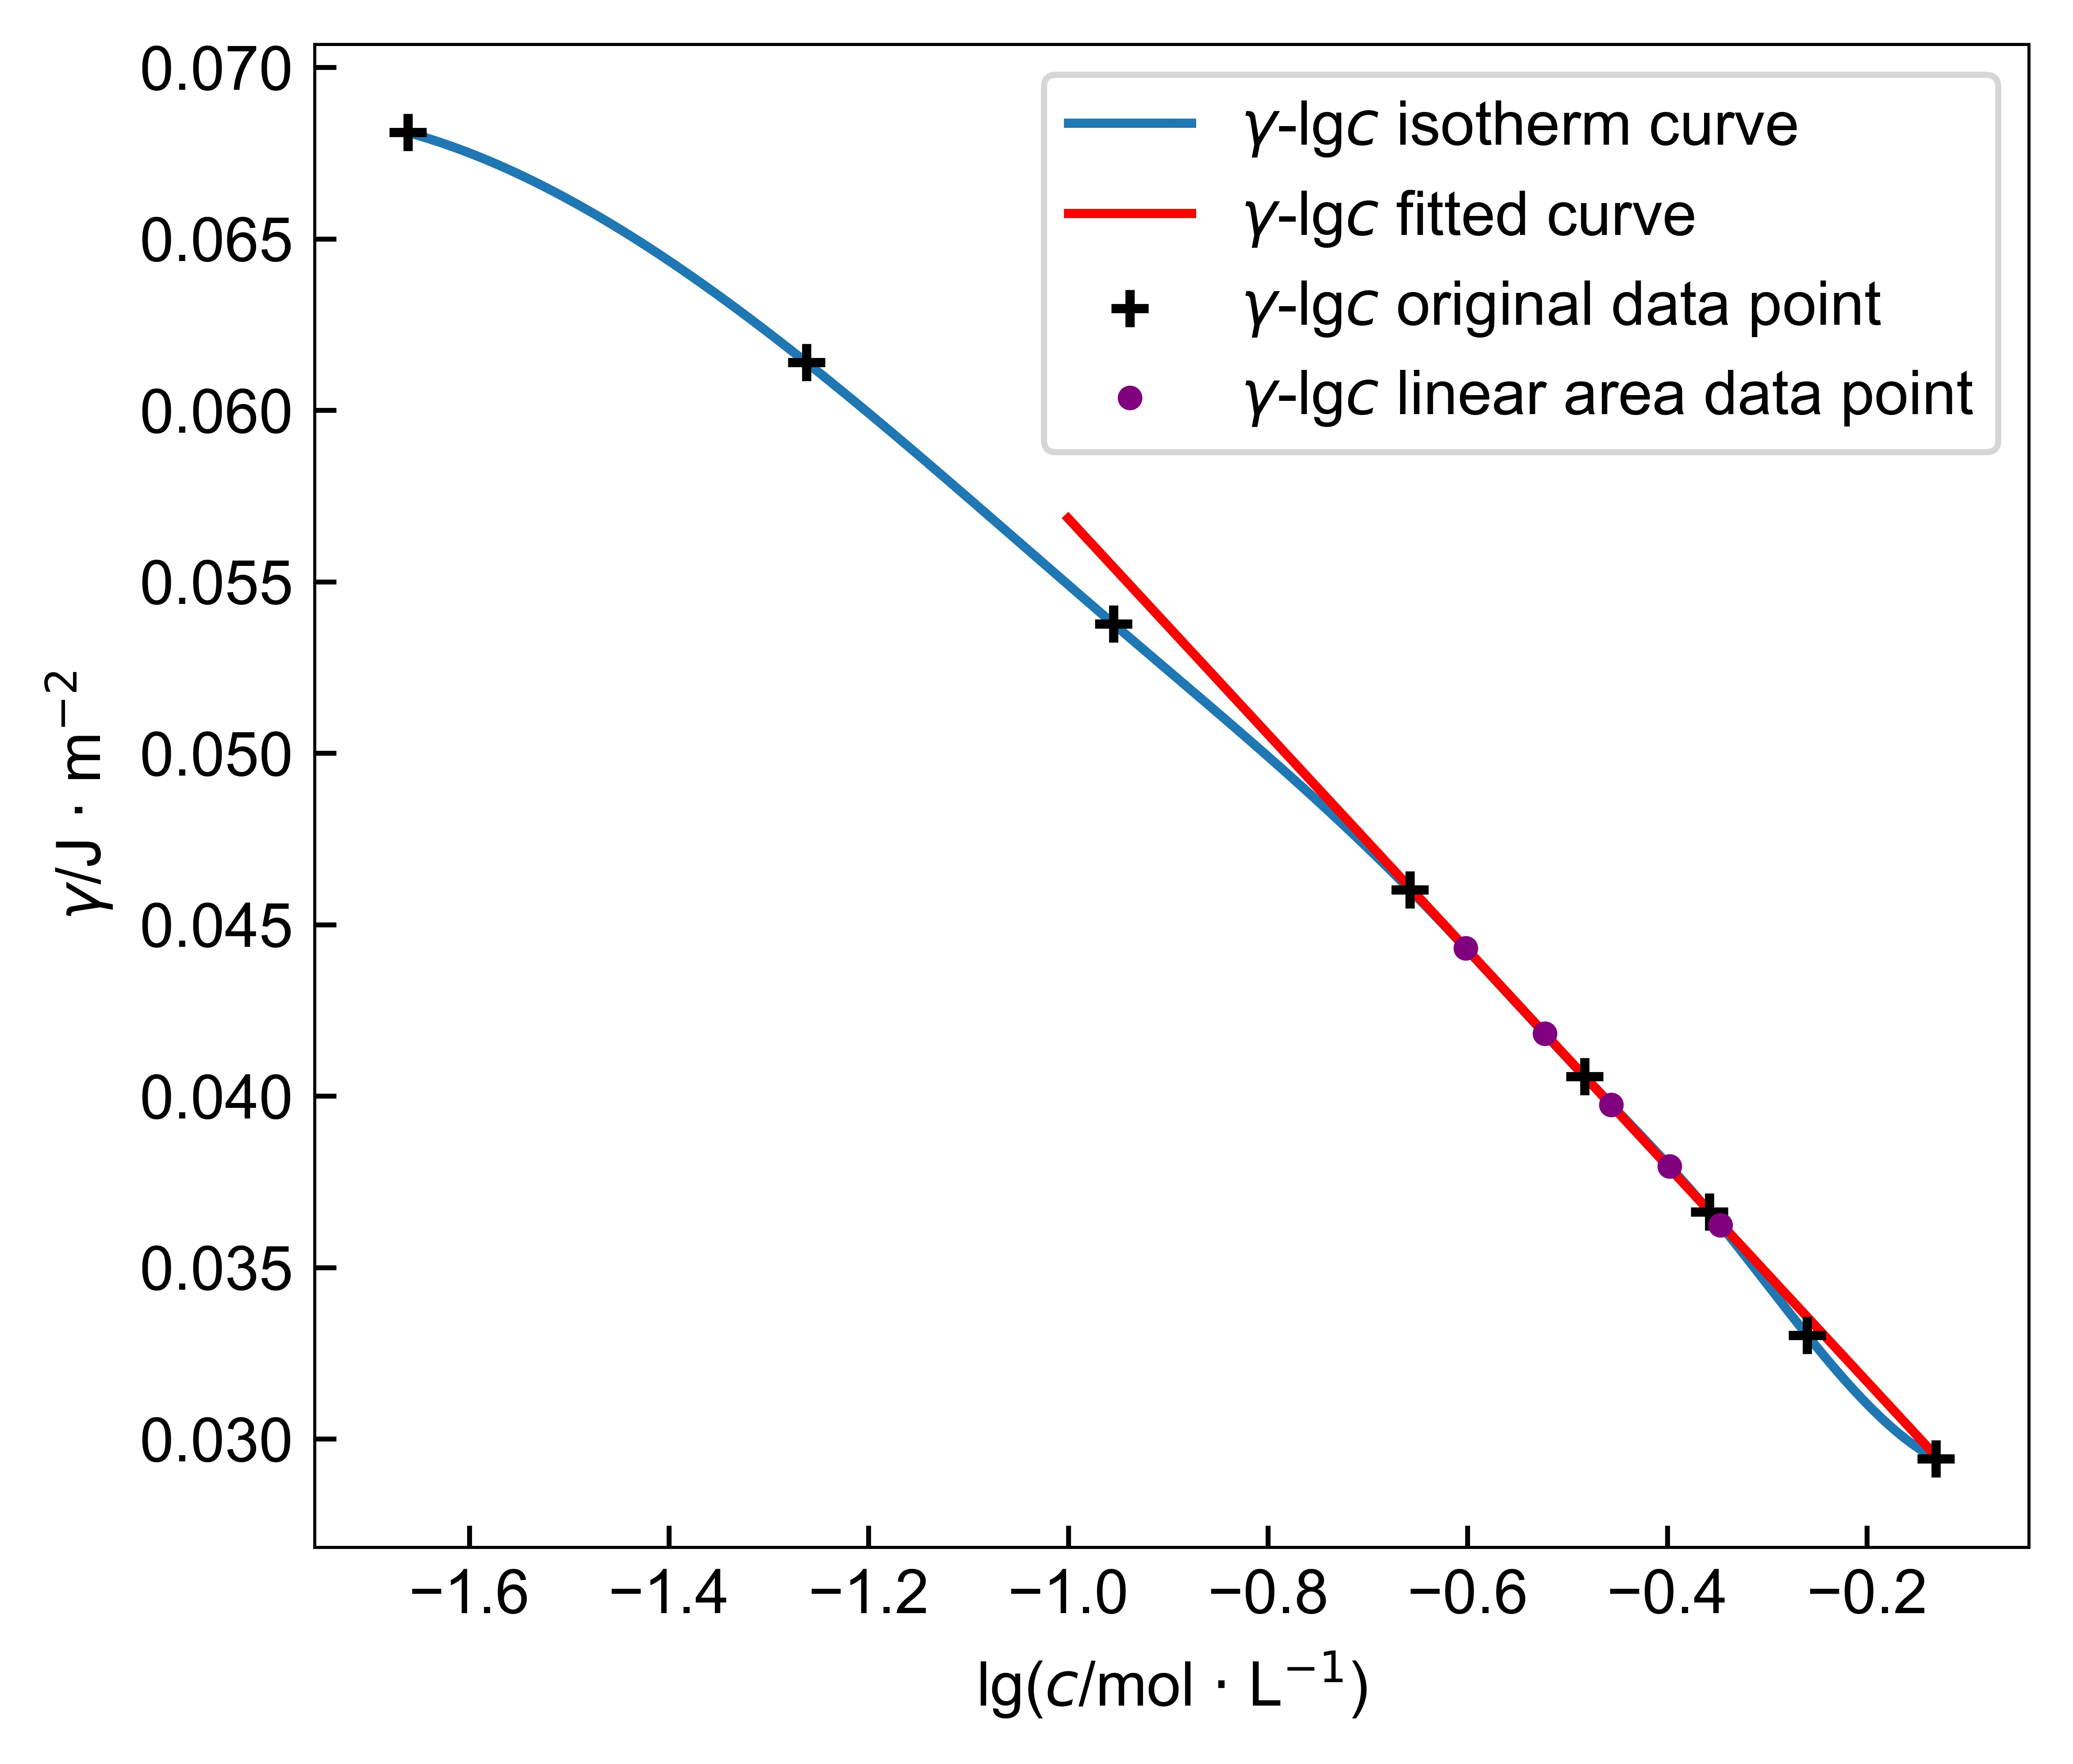
\includegraphics[width=0.65\textwidth]{1.jpg}
	\bicaption{正丁醇水溶液$\gamma-{\rm lg}c$等温曲线及拟合直线}{$\gamma -{\rm lg}c$ isotherm and fitted curve of n-BuOH aqueous solution}
\end{figure}
\par
根据\textbf{图1}可以看出,随着正丁醇浓度$c_{\rm BuOH}$逐渐增大,开始时$\gamma$随${\rm lg}c$的增加下降很慢,呈非线性关系;随后则变化较快,在高于$0.220\ \ {\rm mol\cdot L^{-1}}$浓度范围内基本呈线性关系。\par 
\vbox{}
\vbox{}
在\textbf{图1}中$\gamma-{\rm lg}c$曲线的线性区取5个点,浓度分别为$0.25$、$0.30$、$0.35$、$0.40$、$0.45\ \ {\rm mol\cdot L^{-1}}$,读取相应的$\gamma$值,各点数据示于\textbf{表6}中。
\begin{table}[h]
	\centering
	\zihao{5}
	\bicaption{$\gamma-{\rm lg}c$曲线线性区取点相关数据}{Point data in the linear area of the $\gamma-{\rm lg}c$ curve}
	\begin{tabular}{ccc}
		\toprule
		$c/{\rm mol\cdot L^{-1}}$ & ${\rm lg}(c/{\rm mol\cdot L^{-1}})$& $\gamma/{\rm J\cdot m^{-2}}$\\
		\midrule
		0.250 & -0.602 & 0.04431 \\
		0.300 & -0.523 & 0.04182\\
		0.350 & -0.456 & 0.03975\\
		0.400 & -0.398 & 0.03795\\
		0.450 & -0.347 & 0.03624\\
		\bottomrule
	\end{tabular}
\end{table}
\par 
根据\textbf{表6}数据,对所取的$\gamma-{\rm lg}c$数据进行线性拟合,得到回归直线;所取数据点与拟合得到的回归直线也示于\textbf{图1}中。线性拟合得到的直线方程为
$$
\frac{\gamma}{{\rm J\cdot m^{-2}}}=-0.03146\ \ {\rm lg}(\frac{c}{{\rm mol\cdot L^{-1}}})+0.02538,\ \ R=-0.99991
$$
可见该线性拟合具有很好的效果,也进一步说明了在较高浓度范围内$\gamma-{\rm lg}c$具有很好的线性关系。值得注意的是,观察\textbf{图1}可以发现,在高浓度区所测量的实验数据点除了倒数第二个数据点$0.550\ \ {\rm mol\cdot L^{-1}}$外,均很好地落在了拟合直线上,这暗示$0.550\ \ {\rm mol\cdot L^{-1}}$数据点可能因为操作失误等原因在测量时出现了较大误差,是可信度较低的数据点。该数据点误差较大的可能原因将在第4部分进行详细讨论。\par 
从拟合直线方程中,求出斜率
$$
\frac{d\gamma}{d{\rm lg}c}=-0.03146\ \ {\rm J\cdot m^{-2}}
$$
斜率k的标准误差根据公式
$$
\sigma_{k}=\sqrt{\frac{n\sigma^{2}_{y}}{n\sum x^{2}_{i}-(\sum x_{i})^{2}}}
$$
得到;代入实际数据,计算得
$$
\sigma_{k}=0.003\ \ {\rm J\cdot m^{-2} }
$$
故
$$
\frac{d\gamma}{d{\rm lg}c}=(-0.031\pm0.003) \ \ {\rm J\cdot m^{-2}}
$$
代入室温$T=293.05\ \ {\rm K}$,计算饱和吸附时的饱和吸附量$\Gamma_{\infty}$值
$$
\Gamma_{\infty}=-\frac{1}{2.303RT}\times\frac{d\gamma}{d{\rm lg}c}=(5.6\pm 0.5)\times10^{-6}\ \ {\rm mol\cdot m^{-2}}
$$
\subsubsection{最大气泡压力法计算分子吸附面积$q$与正丁醇分子实际面积$q_{c}$}
计算每个正丁醇分子在溶液表面所占的面积
$$
q=\frac{1}{\Gamma_{\infty}N_{A}}=2.96\times10^{-19}\ \ {\rm m^2}=0.296\ \ {\rm nm^{2}}
$$
标准偏差
$$
\sigma_{q}=\frac{\sigma_{\Gamma_{\infty}}}{\Gamma^{2}_{\infty} N_{A}}=3\times10^{-20}\ \ {\rm m^{2}}=0.03\ \ {\rm nm^{2}}
$$
故
$$
q=(0.30\pm 0.03)\ \ {\rm nm^{2}}
$$
\par 
因为$\Gamma$实际上是一个过剩量,即使其等于0(无吸附),表面上仍有溶质分子,故计算$q$时忽略了表面上原有的溶质分子。对于较浓的溶液,在计算表面上溶质分子数时,除了吸附分子还应考虑原有分子。若$\Gamma$以$\rm mol\cdot m^{-2}$为单位,$c$以$\rm mol\cdot dm^{-3}$为单位,$q_{c}$以$\rm nm^{2}$为单位,则实际溶液浓度为$c$时的吸附量
$$
q_{c}=\frac{10^{18}}{\Gamma N_{A}+100\times(cN_{A})^{2/3}}
$$
以$c=0.329\ \ {\rm mol\cdot L^{-1}}$的正丁醇溶液为例,由\textbf{图1}可以看出,该浓度下切线斜率可以认为与拟合直线斜率相等,$\Gamma=\Gamma_{\infty}$,计算得$\sigma_{q_{c}}=0.03\ \ {\rm nm^{2}}$,代入公式进行计算
$$
q_{c}=\frac{10^{18}}{\Gamma_{\infty} N_{A}+100\times(cN_{A})^{2/3}}=(0.27\pm 0.03)\ \ {\rm nm^{2}}
$$
即为该浓度下正丁醇分子在表面上的实际面积。其他浓度下的计算是类似的。
\subsubsection{吊片法测量正丁醇$\gamma-{\rm lg}c$曲线、饱和吸附量$\Gamma_{\infty}$、分子吸附面积$q$与正丁醇分子实际面积$q_{c}$}
根据\textbf{表4}数据,使用python matplotlib作出正丁醇水溶液$\gamma-{\rm lg}c$关系散点图,并通过SciPy库用3次样条插值曲线光滑连接各散点,形成正丁醇水溶液$\gamma-{\rm lg}c$等温曲线,如\textbf{图2}所示。
\begin{figure}[h]
	\centering
	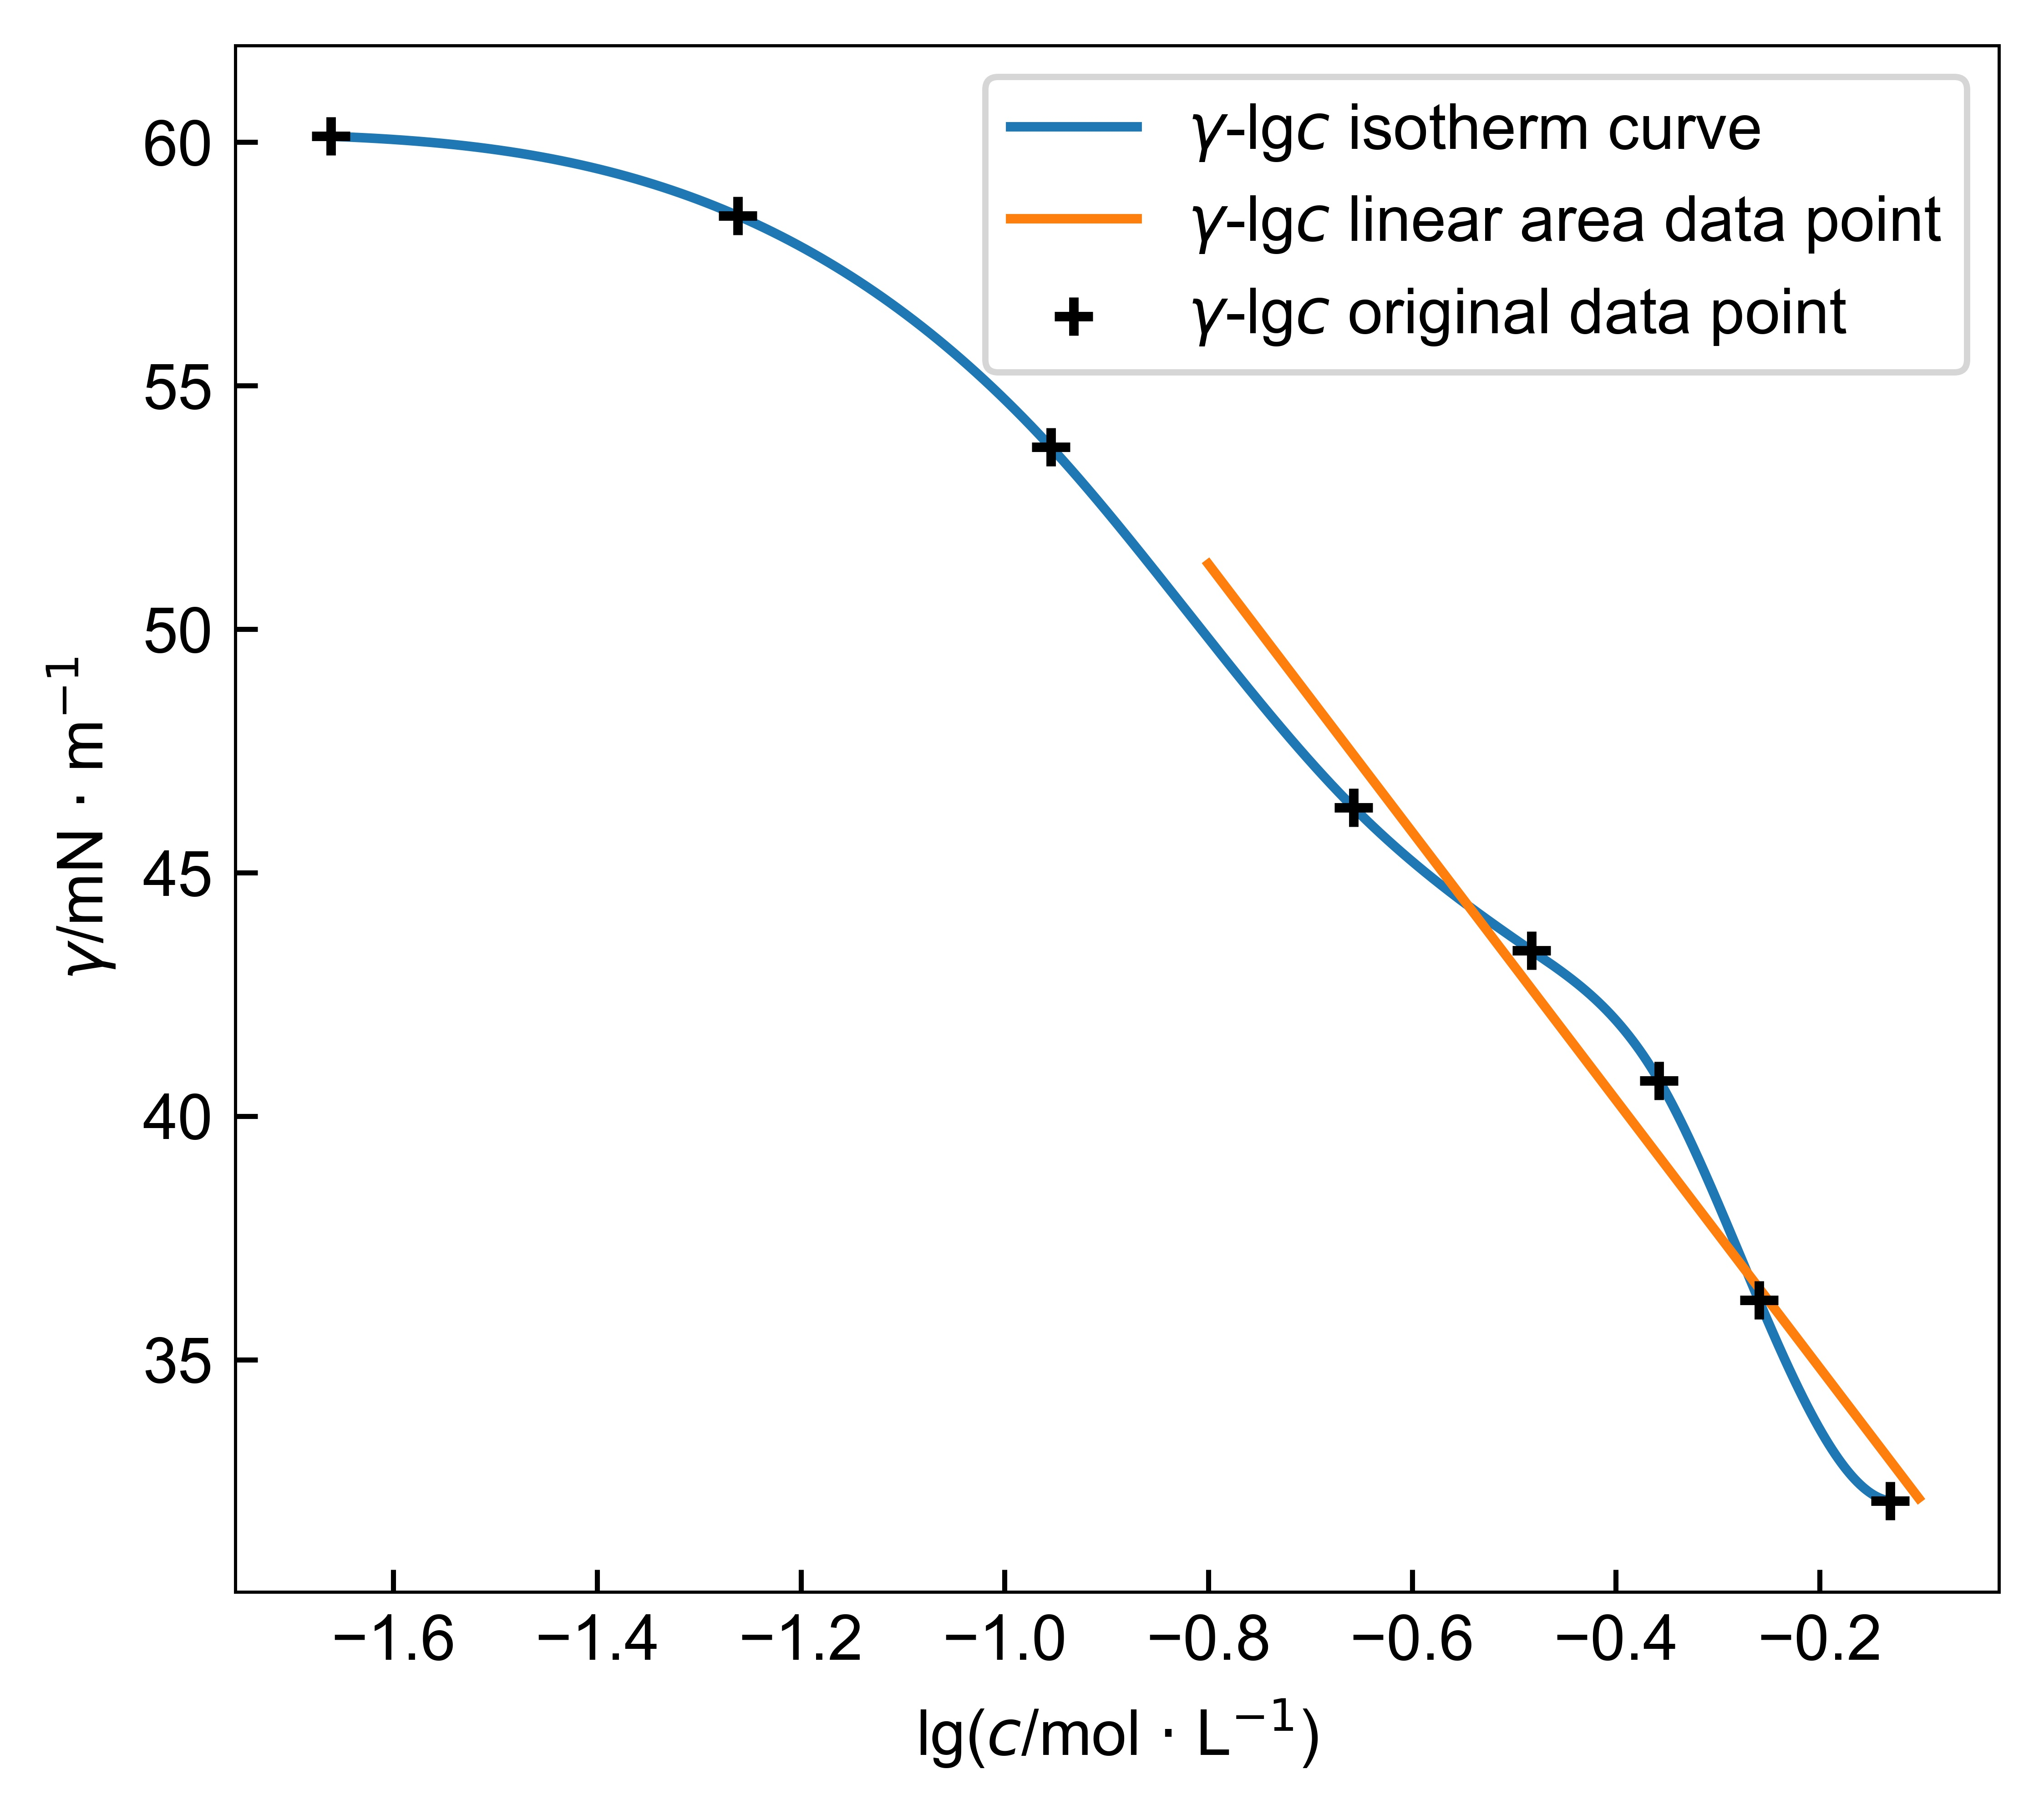
\includegraphics[width=0.65\textwidth]{2.jpg}
	\bicaption{吊片法测量正丁醇水溶液$\gamma-{\rm lg}c$等温曲线}{$\gamma -{\rm lg}c$ isotherm of n-BuOH aqueous solution via hanging-piece method}
\end{figure}
\par
类似地,对$\gamma-{\rm lg}c$曲线近线性区的数据点(第$4\sim 8$组)进行线性拟合,所得回归直线也示于\textbf{图2}中。线性拟合得到的直线方程为
$$
\frac{\gamma}{{\rm J\cdot m^{-2}}}=-(0.028 \pm 0.003 )\ \ {\rm lg}(\frac{c}{{\rm mol\cdot L^{-1}}})+(0.029\pm 0.001),\ \ R=-0.97991
$$
根据拟合直线的斜率
$$
\frac{d\gamma}{d{\rm lg}c}=-(0.028\pm 0.003)\ \ {\rm J\cdot m^{-2}}
$$
代入室温$T=293.05\ \ {\rm K}$,计算饱和吸附时的饱和吸附量$\Gamma_{\infty}$值
$$
\Gamma_{\infty}=-\frac{1}{2.303RT}\times\frac{d\gamma}{d{\rm lg}c}=(5.0\pm 0.5)\times10^{-6}\ \ {\rm mol\cdot m^{-2}}
$$
\par 
计算每个正丁醇分子在溶液表面所占的面积
$$
q=\frac{1}{\Gamma_{\infty}N_{A}}=3.32\times10^{-19}\ \ {\rm m^2}=0.332\ \ {\rm nm^{2}}
$$
标准偏差
$$
\sigma_{q}=\frac{\sigma_{\Gamma_{\infty}}}{\Gamma^{2}_{\infty} N_{A}}=3\times10^{-20}\ \ {\rm m^{2}}=0.03\ \ {\rm nm^{2}}
$$
故
$$
q=(0.33\pm 0.03)\ \ {\rm nm^{2}}
$$
\par 
因为$\Gamma$实际上是一个过剩量,即使其等于0(无吸附),表面上仍有溶质分子,故计算$q$时忽略了表面上原有的溶质分子。对于较浓的溶液,在计算表面上溶质分子数时,除了吸附分子还应考虑原有分子。若$\Gamma$以$\rm mol\cdot m^{-2}$为单位,$c$以$\rm mol\cdot dm^{-3}$为单位,$q_{c}$以$\rm nm^{2}$为单位,则实际溶液浓度为$c$时的吸附量
$$
q_{c}=\frac{10^{18}}{\Gamma N_{A}+100\times(cN_{A})^{2/3}}
$$
以$c=0.329\ \ {\rm mol\cdot L^{-1}}$的正丁醇溶液为例,由\textbf{图2}可以看出,该浓度下切线斜率可以认为与拟合直线斜率相等,$\Gamma=\Gamma_{\infty}$,计算得$\sigma_{q_{c}}=0.03\ \ {\rm nm^{2}}$,代入公式进行计算
$$
q_{c}=\frac{10^{18}}{\Gamma_{\infty} N_{A}+100\times(cN_{A})^{2/3}}=(0.30\pm 0.03)\ \ {\rm nm^{2}}
$$
即为该浓度下正丁醇分子在表面上的实际面积。其他浓度下的计算是类似的。
\par 

对比\textbf{图1}和\textbf{图2}可以看出,吊片法测量得到的$\gamma-{\rm lg}c$等温曲线在高浓度区也未呈现很好的线性关系,说明吊片法测量正丁醇表面张力的误差相对较大。



 
 	 \section{讨论与结论}
		\subsection{实验讨论}
 			\subsubsection{造成测量误差的原因分析}
如3.2.2所述,根据\textbf{图1}曲线形状,可以初步判断倒数第二组溶液的表面张力测量出现了较大误差。回忆实验的实际过程,可能的原因分析如下:\par 
其一,由于该正丁醇溶液浓度较高,溶液黏度大,具有较强的表面活性剂特性;在打开活塞后,毛细管尖端“吹出”的一团气泡一段时间内无法散去,此时未能及时注意到该现象而继续进行实验,使毛细管尖端不能直接接触液面,造成一定的测量误差。对此,应当用手指轻弹小试管,待气泡消失后再进行下一步测量。\par 
其二,毛细管尖端未充分接触凹液面最低处,产生侧向表面张力,造成测量误差。由于正丁醇溶液的表面张力,毛细管尖端靠近液面的过程中,刚刚接触液面时产生液面向上隆起、“迎合”毛细管尖端的现象。对此,应当从小试管侧下方观察,确保毛细管尖端位于实际液面最低处,与液面相切。\par 
以上两个原因也是本次实验能否成功、测量是否足够准确的重要决定因素。
 	 	\subsubsection{实验改进}
考虑到最大气泡压力法测量表面张力过程中压力计左右两端水柱高度变化速度较快,可能因测量者反应不及造成一定的读数误差,可以对该实验装置进行一定的自动化改装,例如加装传感器等以自动探测液面高度变化,从而减小实验误差。 


 	 \subsection{实验结论}
本次实验通过两种不同的实验方法对溶液的表面张力和表面吸附进行了测定,使用最大气泡压力法和吊片法测定纯水和8个不同浓度正丁醇溶液的表面张力,分别作出了两种方法得到的正丁醇水溶液的$\gamma-{\rm lg}c$等温曲线,比较了两方法得到的曲线的差异。\par 
根据最大气泡压力法得到的$\gamma-{\rm lg}c$等温曲线线性区斜率,计算了正丁醇分子的饱和吸附量$\Gamma_{\infty}=(5.6\pm 0.5)\times10^{-6}\ \ {\rm mol\cdot m^{-2}}$,分子吸附面积$q=(0.30\pm 0.03)\ \ {\rm nm^{2}}$,$c=0.329\ \ {\rm mol\cdot L^{-1}}$的正丁醇溶液分子实际面积$q_{c}=(0.27\pm 0.03)\ \ {\rm nm^{2}}$。根据吊片法得到的$\gamma-{\rm lg}c$等温曲线线性区斜率,计算了正丁醇分子的饱和吸附量$\Gamma_{\infty}=(5.0\pm 0.5)\times10^{-6}\ \ {\rm mol\cdot m^{-2}}$,分子吸附面积$q=(0.33\pm 0.03)\ \ {\rm nm^{2}}$,$c=0.329\ \ {\rm mol\cdot L^{-1}}$的正丁醇溶液分子实际面积$q_{c}=(0.30\pm 0.03)\ \ {\rm nm^{2}}$并探讨了造成实验误差的原因。\par 
通过本次实验,充分运用了Gibbs吸附公式计算了溶液表面吸附量和饱和吸附时每个分子所占表面面积,初步了解了测量溶液表面张力的常用方法。

 

   
\vbox{}
\vbox{}

\bibliographystyle{achemso}
\bibliography{b}



\end{document}